\documentclass{beamer}                             % presentation
% \documentclass[draft]{beamer}                    % improves compile time
\usepackage[utf8]{inputenc}                        % utf8
\usepackage[T1]{fontenc}                           % fix font encoding
\usepackage[english]{babel}                        % language
\usepackage[autostyle, english=american]{csquotes} % quotes
\usepackage{amsmath, amssymb, amsthm}              % ams mathematical packages
\usepackage{physics, mathtools, bm}                % extra math packages
\usepackage{graphicx, subcaption}                  % images
\usepackage{tikz, pgfplots}                        % plots and graphs
\usepackage[style=ieee]{biblatex}                  % bibliography
\usepackage{geometry, hyperref, enumitem}          % misc.

\usetikzlibrary{positioning}                       % advanced positioning
\pgfplotsset{compat=newest}                        % version of pgfplots

\graphicspath{{./figures/}}
\addbibresource{references.bib}

% TODO: fix plot (KL-divergence to kl divergence, 2x bug, etc.)
% TODO: use svg plots from matplotlib

\renewcommand{\vec}[1]{\bm{#1}}

% serif font in math mode
% https://ctan.math.utah.edu/ctan/tex-archive/fonts/lm/tex/latex/lm/lmodern.sty
% \usefonttheme[onlymath]{serif}
\renewcommand\mathfamilydefault{cmr}

\SetSymbolFont{operators}   {normal}{OT1}{cmr} {m}{n}
\SetSymbolFont{letters}     {normal}{OML}{cmm} {m}{it}
\SetSymbolFont{symbols}     {normal}{OMS}{cmsy}{m}{n}
\SetSymbolFont{largesymbols}{normal}{OMX}{cmex}{m}{n}
\SetSymbolFont{operators}   {bold}  {OT1}{cmr} {bx}{n}
\SetSymbolFont{letters}     {bold}  {OML}{cmm} {b}{it}
\SetSymbolFont{symbols}     {bold}  {OMS}{cmsy}{b}{n}
\SetSymbolFont{largesymbols}{bold}  {OMX}{cmex}{m}{n}

\SetMathAlphabet{\mathbf}{normal}{OT1}{cmr}{bx}{n}
\SetMathAlphabet{\mathsf}{normal}{OT1}{cmss}{m}{n}
\SetMathAlphabet{\mathit}{normal}{OT1}{cmr}{m}{it}
\SetMathAlphabet{\mathtt}{normal}{OT1}{cmtt}{m}{n}
\SetMathAlphabet{\mathbf}{bold}  {OT1}{cmr}{bx}{n}
\SetMathAlphabet{\mathsf}{bold}  {OT1}{cmss}{bx}{n}
\SetMathAlphabet{\mathit}{bold}  {OT1}{cmr}{bx}{it}
\SetMathAlphabet{\mathtt}{bold}  {OT1}{cmtt}{m}{n}

% customize \item in itemize
\setitemize{label={},itemsep=0.5cm}

\renewcommand{\vec}[1]{\bm{#1}}

\DeclareMathOperator{\diag}{diag}
\DeclareMathOperator{\logdet}{logdet}
\DeclareMathOperator{\chol}{chol}

\DeclareMathOperator*{\argmax}{argmax}
\DeclareMathOperator*{\argmin}{argmin}

\DeclareMathOperator{\E}{E}
\DeclareMathOperator{\Var}{Var}
\DeclareMathOperator{\Cov}{Cov}
\DeclareMathOperator{\info}{I}
\DeclareMathOperator{\entropy}{H}

%%% colors

\definecolor{lightblue}{HTML}{a1b4c7}
\definecolor{orange}{HTML}{ea8810}
\definecolor{silver}{HTML}{b0aba8}
\definecolor{rust}{HTML}{b8420f}
\definecolor{seagreen}{HTML}{23553c}

\colorlet{lightsilver}{silver!20!white}
\colorlet{darkorange}{orange!85!black}
\colorlet{darksilver}{silver!85!black}
\colorlet{darklightblue}{lightblue!75!black}
\colorlet{darkrust}{rust!85!black}
\colorlet{darkseagreen}{seagreen!85!black}

\hypersetup{
  colorlinks=true,
  linkcolor=darkrust,
  citecolor=darkseagreen,
  urlcolor=darksilver
}

%%% beamer settings

\usetheme{Pittsburgh}
\usecolortheme{dolphin}

% hide navigation buttons
\setbeamertemplate{navigation symbols}{}
% change title color
\setbeamercolor{title}{fg=darklightblue}
\setbeamercolor{frametitle}{fg=darklightblue}
% change bibliography entry colors
\setbeamercolor{bibliography entry author}{fg=darklightblue}
\setbeamercolor{bibliography entry note}{fg=lightblue}

% title page
\title[]{Fast Gaussian process regression by \\ Greedy Conditional Selection}
\subtitle{}
\author[Huan, Sch{\"a}fer]
{Stephen Huan \and Florian\ Sch{\"a}fer}
\institute[Georgia Institute of Technology]
{
  Short \& Sweet seminar
}
\date[]{April 22, 2022}
\subject{Computer Science}

\begin{document}
\frame{\titlepage}

\begin{frame}
\frametitle{The problem: Gaussian process regression}
\framesubtitle{}
  \begin{columns}
    \begin{column}{0.6\textwidth}
      \begin{itemize}
        \item<+-> Measurements \( \vec{y}_\text{Tr} \) at
          \( N \) points \( X_\text{Tr} \)

        \item<+-> Estimate unseen data \(
          \vec{y}_\text{Pr} \) at \( X_\text{Pr} \)

        \item<+-> Model as Gaussian process

          \( \rightarrow \) condition on \( \vec{y}_\text{Tr} \)
      \end{itemize}
    \end{column}
    \begin{column}{0.4\textwidth}
      \begin{figure}
        \centering
        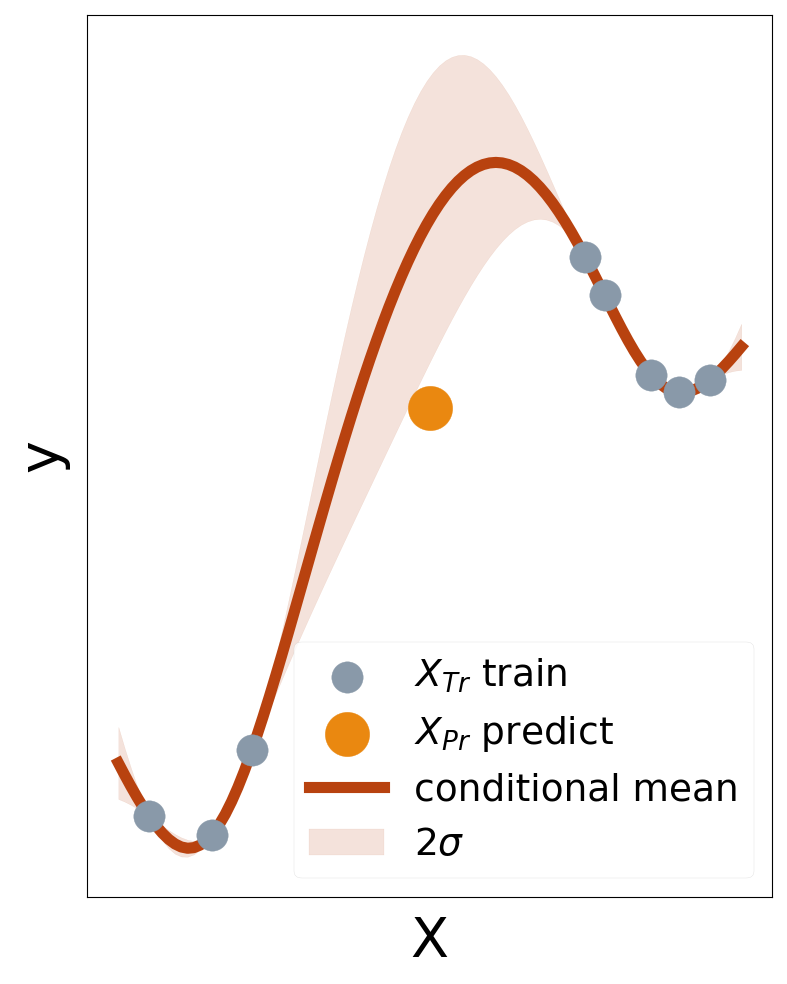
\includegraphics[width=\textwidth]{graphs/predict_all}
      \end{figure}
    \end{column}
  \end{columns}
\end{frame}

\begin{frame}
\frametitle{Cubic bottleneck}
\framesubtitle{}
\begin{itemize}
  \item<+-> Closed-form conditional distribution:
    \begin{align*}
      \E[\vec{y}_\text{Pr} \mid \vec{y}_\text{Tr}] &=
        \vec{\mu}_\text{Pr} +
        \Theta_{\text{Pr}, \text{Tr}} \Theta_{\text{Tr}, \text{Tr}}^{-1}
        (\vec{y}_\text{Tr} - \vec{\mu}_\text{Tr}) \\
      \Theta_{\text{Pr}, \text{Pr} \mid \text{Tr}} :=
      \Cov[\vec{y}_\text{Pr} \mid \vec{y}_\text{Tr}] &=
        \Theta_{\text{Pr}, \text{Pr}} -
        \Theta_{\text{Pr}, \text{Tr}} \Theta_{\text{Tr}, \text{Tr}}^{-1}
        \Theta_{\text{Tr}, \text{Pr}}
    \end{align*}
  \item<+-> Kernel function \( K(\cdot, \cdot) \):
    \( \Theta_{i, j} := K(\vec{x}_i, \vec{x}_j) \)

  \item<+-> Computational cost scales as \( N^3 \)
\end{itemize}
\end{frame}

\begin{frame}
\frametitle{Screening effect}
\framesubtitle{}

\begin{columns}
  \begin{column}{0.6\textwidth}
    \begin{itemize}
      \item<+-> ``Screening effect''
      \item<+-> Choose \( k \) \textcolor{lightblue}{most informative} points
    \end{itemize}
  \end{column}
  \begin{column}{0.4\textwidth}
      \begin{figure}
        \centering
        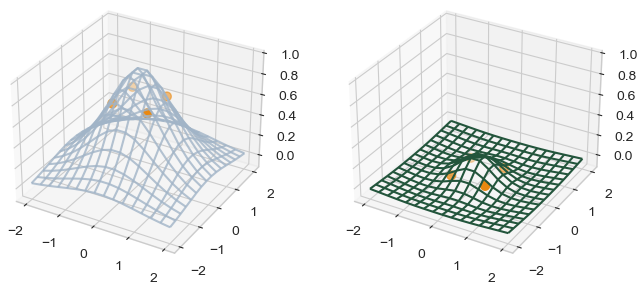
\includegraphics[width=\textwidth]{kernel2d}
      \end{figure}
  \end{column}
\end{columns}
\end{frame}

\begin{frame}
\frametitle{Conditional \( k \)-th nearest neighbors}
\framesubtitle{}

\begin{columns}
  \begin{column}{0.6\textwidth}
    \begin{itemize}
      \item<1-> Naive: select \( k \) closest points

      \item<2-> Chooses redundant information

      \item<3-> Maximize \emph{mutual information}!
    \end{itemize}
  \end{column}
  \begin{column}{0.4\textwidth}

    \only<1>{
      \begin{figure}
        \centering
        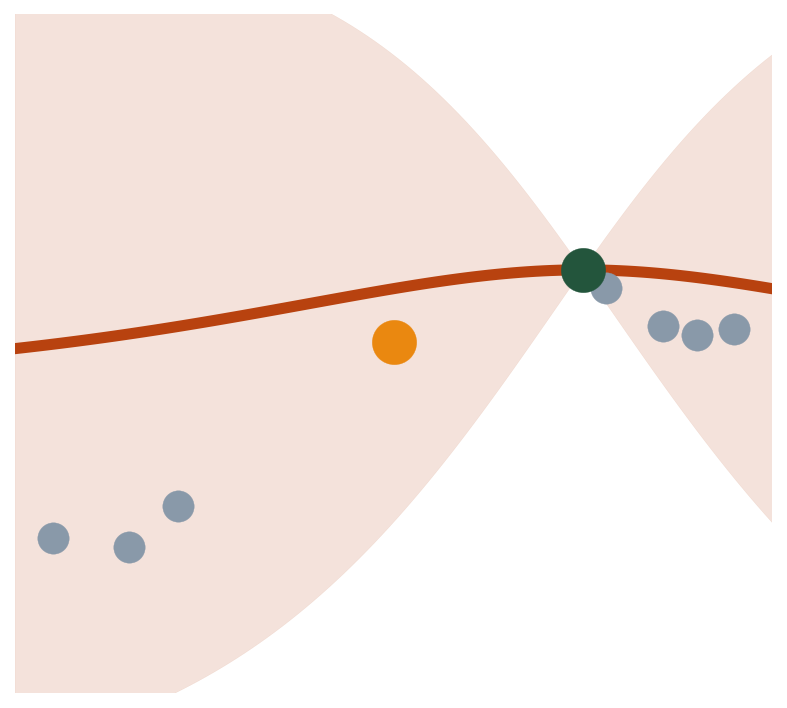
\includegraphics[width=\textwidth]{graphs/predict_knn_1}
      \end{figure}
    }

    \only<2->{
      \begin{figure}
        \centering
        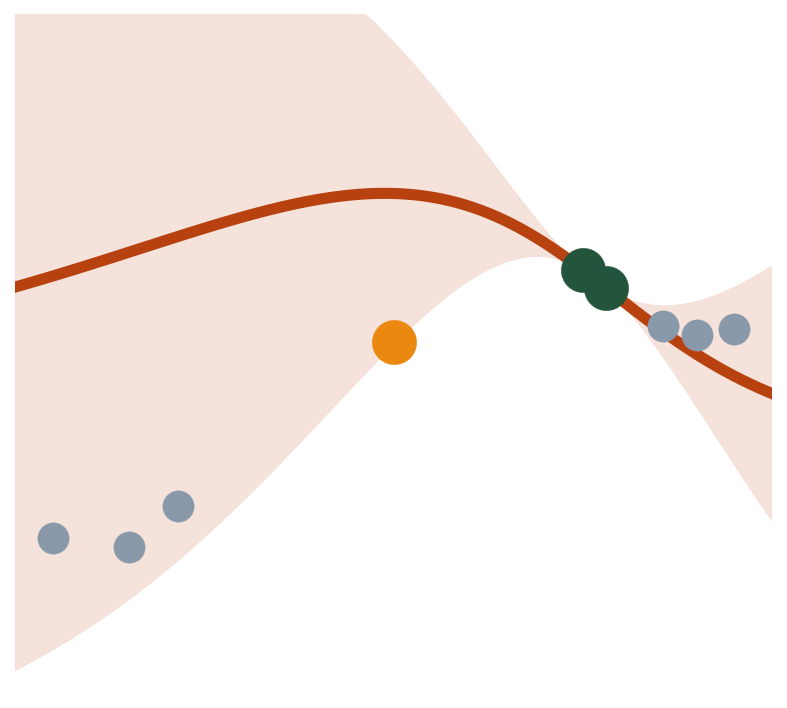
\includegraphics[width=\textwidth]{graphs/predict_knn_2}
      \end{figure}
    }

    \vspace{-0.6cm}

    \uncover<3-> {
      \only<-3>{
        \begin{figure}
          \centering
          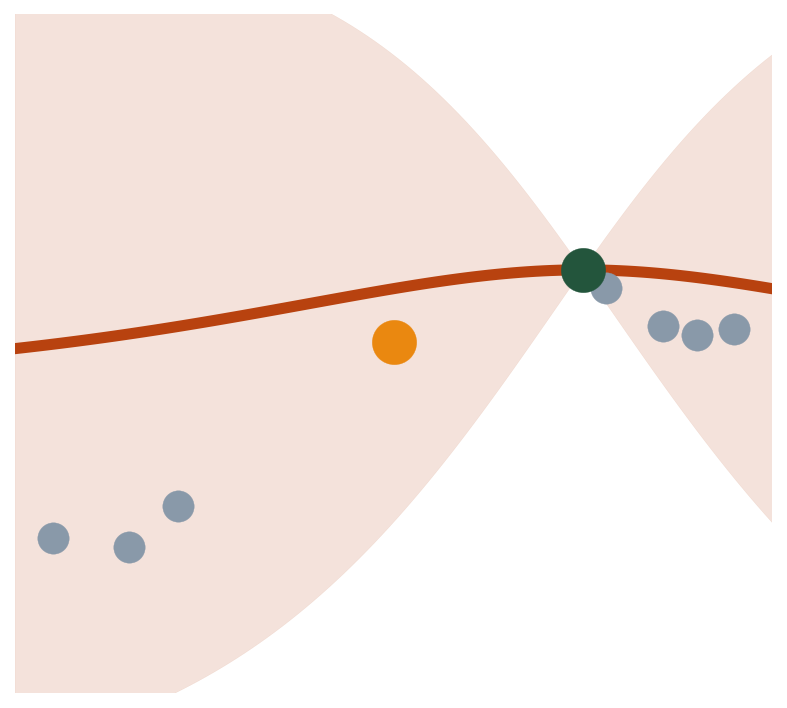
\includegraphics[width=\textwidth]{graphs/predict_cknn_1}
        \end{figure}
      }

      \only<4-> {
        \begin{figure}
          \centering
          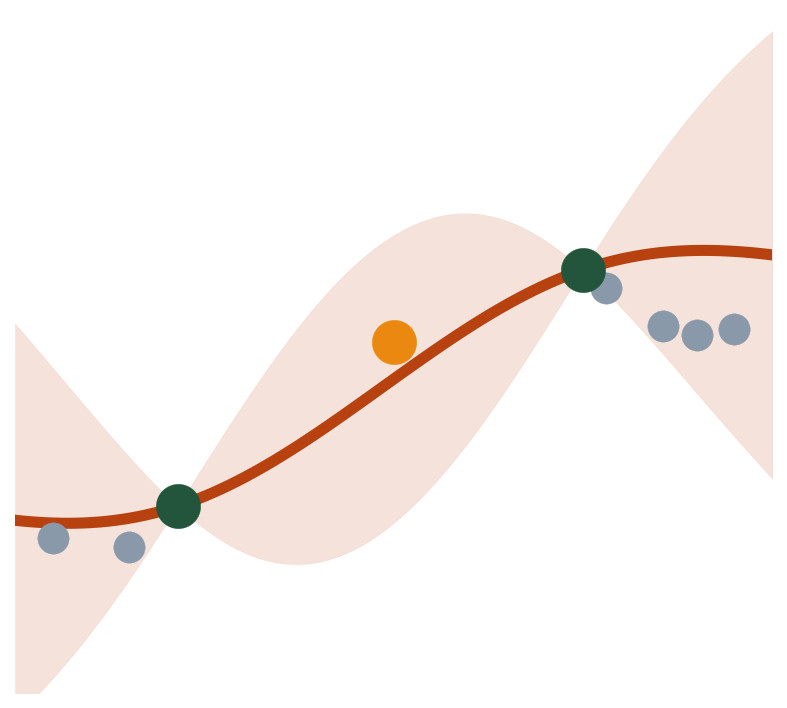
\includegraphics[width=\textwidth]{graphs/predict_cknn_2}
        \end{figure}
      }
    }

  \end{column}
\end{columns}
\end{frame}

\begin{frame}
\frametitle{Mutual information}
\framesubtitle{}

\begin{itemize}
  \item<+-> Mutual information or information gain:
    \begin{align*}
      \info[\vec{y}_\text{Pr};\vec{y}_\text{Tr}] &=
        \entropy[\vec{y}_\text{Pr}] -
        \entropy[\vec{y}_\text{Pr} \mid \vec{y}_\text{Tr}]
    \end{align*}
  \item<+-> Entropy increases with log determinant of covariance
  \item<+-> Information-theoretic EV-VE identity:
    \begin{align*}
      \textcolor{orange}{\entropy[\vec{y}_\text{Pr}]} &=
        \textcolor{lightblue}{
          \entropy[\vec{y}_\text{Pr} \mid \vec{y}_\text{Tr}]
        } +
        \textcolor{rust}{\info[\vec{y}_\text{Pr};\vec{y}_\text{Tr}]} \\
      \textcolor{orange}{\Var[\vec{y}_\text{Pr}]} &=
        \textcolor{lightblue}{
          \E[\Var[\vec{y}_\text{Pr} \mid \vec{y}_\text{Tr}]]
        } +
        \textcolor{rust}{\Var[\E[\vec{y}_\text{Pr} \mid \vec{y}_\text{Tr}]]}
    \end{align*}
\end{itemize}
\end{frame}

\begin{frame}
\frametitle{Greedy mutual information maximization}
\framesubtitle{}
\begin{itemize}
  \item<+-> Greedy selection, maintain selected indices \( I \)
  \item<+-> Criterion simplifies to:
    \begin{align*}
        \argmax_{j \not \in I} \:
          \frac{\Theta_{j, \text{Pr} \mid I}^2}{\Theta_{j, j \mid I}}
    \end{align*}
  \item<+-> Direct computation: \( \mathcal{O}(N k^4) \)
  \item<+-> Storing a partial Cholesky factor: \( \mathcal{O}(N k^2) \)
\end{itemize}
\end{frame}

\begin{frame}
\frametitle{Conditioning as rank-one update}
\framesubtitle{}
\begin{itemize}
  \item<+-> Key idea: assume we have \( \Theta_{\mid I} \),
    rank-one update to \( \Theta_{\mid I \cup \{ k \}} \)
    \begin{align*}
      \Theta_{:, : \mid I \cup \{ k \}} &= \Theta_{:, : \mid I} -
        \Theta_{:, k \mid I} \Theta_{k, k \mid I}^{-1} \Theta_{k, : \mid I} \\
      \vec{u} &= \frac{\Theta_{:, k \mid I}}{\sqrt{\Theta_{k, k \mid I}}} \\
      \Theta_{\mid I \cup \{ k \}} &= \Theta_{\mid I} - \vec{u} \vec{u}^{\top}
    \end{align*}
\end{itemize}
\end{frame}

\begin{frame}
\frametitle{Efficient computation from Cholesky factor}
\framesubtitle{}
\begin{itemize}
  \item<+-> Statistical interpretation of Cholesky factorization:
    {\footnotesize
      \begin{align*}
        \chol(\Theta) &=
        \begin{pmatrix}
          I & 0 \\
          \textcolor{darkorange}{\Theta_{2, 1} \Theta_{1, 1}^{-1}} & I
        \end{pmatrix}
        \begin{pmatrix}
          \chol(\Theta_{1, 1}) & 0 \\
          0 & \chol(\textcolor{lightblue}{
            \Theta_{2, 2} - \Theta_{2, 1} \Theta_{1, 1}^{-1} \Theta_{1, 2}
          })
        \end{pmatrix} \\
        &=
        \begin{pmatrix}
          \chol(\Theta_{1, 1}) & 0 \\
          \Theta_{2, 1} \chol(\Theta_{1, 1})^{-\top} & \chol(
            \Theta_{2, 2} - \Theta_{2, 1} \Theta_{1, 1}^{-1} \Theta_{1, 2}
          )
        \end{pmatrix}
      \end{align*}
    }
  \item<+-> Store partial Cholesky factor \( L \)
    \begin{align*}
      L_i = \frac{\Theta_{:, k \mid :i}}{\sqrt{\Theta_{kk \mid :i}}} \\
    \end{align*}
\end{itemize}
\end{frame}

\begin{frame}
\frametitle{Algorithm}
\framesubtitle{}
\begin{itemize}
  \item<+-> Indices \( I \), select \( k \), \( i \)th iteration, have:
    \begin{itemize}
      \item Conditional covariances \( \Theta_{:, \text{Pr} \mid I} \)
      \item Conditional variances \( \diag(\Theta_{:, : \mid I}) \)
      \item First \( i - 1 \) columns of \( L \)
    \end{itemize}
  \item<+-> Update \( L \)
    \begin{align*}
        L_{:, i} \gets
          \Theta_{:, k} - L_{:, :i - 1} L_{k, :i - 1}^{\top}
    \end{align*}
  \item<+-> Update conditional values for candidate \( j \)
    \begin{align*}
      \Theta_{jj \mid I \cup \{ k \}} &\gets
        \Theta_{jj \mid I} - L_{j, i}^2 \\
      \Theta_{j, \text{Pr} \mid I \cup \{ k \}} &\gets
        \Theta_{j, \text{Pr} \mid I} - L_{j, i} L_{\text{Pr}, i}
    \end{align*}
\end{itemize}
\end{frame}

\begin{frame}
\frametitle{Extending to multiple prediction points}
\framesubtitle{}
\begin{itemize}
  \item<+-> Objective conditional log determinant of prediction points
    \begin{align*}
      \logdet
      \left (
        \Theta_{\text{Pr}, \text{Pr} \mid I \cup \{ k \}}
      \right ) = \logdet
        \left (
          \Theta_{\text{Pr}, \text{Pr} \mid I} -
          \frac{\Theta_{\text{Pr}, k \mid I}
                \Theta_{\text{Pr}, k \mid I}^{\top}
              }{\Theta_{kk \mid I}}
        \right )
    \end{align*}
  \item<+-> By the matrix determinant lemma,
    \begin{align*}
      &= \logdet \left ( \Theta_{\text{Pr}, \text{Pr} \mid I} \right ) +
        \log
        \left (
          1 -
          \frac{\Theta_{\text{Pr}, k \mid I}^{\top}
                \Theta_{\text{Pr}, \text{Pr} \mid I}^{-1}
                \Theta_{\text{Pr}, k \mid I}
              }{\Theta_{kk \mid I}}
        \right ) \\
      &= \logdet \left ( \Theta_{\text{Pr}, \text{Pr} \mid I} \right ) +
        \log
        \left (
          \frac{\Theta_{kk \mid I} -
                \Theta_{k, \text{Pr} \mid I}
                \Theta_{\text{Pr}, \text{Pr} \mid I}^{-1}
                \Theta_{\text{Pr}, k \mid I}
              }{\Theta_{kk \mid I}}
        \right )
    \end{align*}
  \item<+-> By the quotient rule, we combine the conditioning:
    \begin{align*}
      &= \logdet \left ( \Theta_{\text{Pr}, \text{Pr} \mid I} \right ) +
        \log
        \left (
          \frac{\Theta_{kk \mid I, \text{Pr}}}{\Theta_{kk \mid I}}
        \right )
    \end{align*}
\end{itemize}
\end{frame}

\begin{frame}
\frametitle{Algorithm for multiple prediction points}
\framesubtitle{}
\begin{itemize}
  \item<+-> Final objective simplifies to:
    \begin{align*}
      \logdet
      \left (
        \Theta_{\text{Pr}, \text{Pr} \mid I \cup \{ k \}}
      \right ) -
      \logdet \left ( \Theta_{\text{Pr}, \text{Pr} \mid I} \right ) &=
      \log
      \left (
        \frac{\Theta_{kk \mid I, \text{Pr}}}{\Theta_{kk \mid I}}
      \right )
    \end{align*}
  \item<+-> Store \emph{two} factors
    (one for numerator, one for denominator)
  \item<+-> ``Pre-condition'' numerator factor on prediction points
    \begin{align*}
      \Theta_{kk \mid I, \text{Pr}} = \Theta_{kk \mid \text{Pr}, I}
    \end{align*}
  \item<+-> Complexity of \( \mathcal{O}(N k^2 +
    N m^2 + m^3) \) for \( m \) prediction points
\end{itemize}
\end{frame}

\begin{frame}
\frametitle{Global approximation by KL-minimization}
\framesubtitle{}
\begin{itemize}
  \item<+-> Approximate GP by sparse Cholesky factor of its precision
  \item<+-> Measure resulting approximation accuracy by KL divergence:
    \begin{align*}
      L \coloneqq \argmin_{\hat{L} \in S} \, \mathbb{D}_{\text{KL}}
        \left (
          \mathcal{N}(\vec{0}, \Theta) \, \Big \| \,
          \mathcal{N}(\vec{0}, (\hat{L} \hat{L}^{\top})^{-1})
        \right )
    \end{align*}
  \item<+-> Using the optimal unique minimizer \( L \) from closed form:
    \begin{align*}
      L_{s_i, i} = \frac{\Theta_{s_i, s_i}^{-1} \vec{e}_1}
      {\sqrt{\vec{e}_1^{\top} \Theta_{s_i, s_i}^{-1} \vec{e}_1}}
    \end{align*}
  \item<+-> Minimize variance of \( i \)th point, conditional on selected!
    \begin{align*}
      2 \mathbb{D}_{\text{KL}}
      &= \sum_{i = 1}^N
        \left [
          \log \left ( \Theta_{ii \mid s_i - \{ i \}} \right ) -
          \log \left ( \Theta_{ii \mid i + 1:} \right )
        \right ]
    \end{align*}
\end{itemize}
\end{frame}

% https://tex.stackexchange.com/questions/518750/beamer-how-to-make-footnote-rule-appear-later-pause
\begingroup
\let\oldfootnoterule\footnoterule
\renewcommand\footnoterule{\only<3->\oldfootnoterule}
\begin{frame}
\frametitle{Cholesky factorization by selection}
\framesubtitle{}

\begin{columns}
  \begin{column}{0.6\textwidth}
    \begin{itemize}
      \item<+-> Apply column-wise directly

      \item<+-> Improves approx. algorithm of \footnotemark
    \end{itemize}
  \end{column}
  \begin{column}{0.4\textwidth}
    \begin{figure}[h!]
      \centering
      \begin{tikzpicture}[scale=1/5]
        % outer triangular factor
\fill[lightsilver] (0, 0) -- (0, -16) -- (16, -16) -- cycle;

% column rectangle
\draw[fill=lightblue] (3, -4) rectangle (4, -16);

% triangular factor
\fill[silver] (0, 0) rectangle (1, -1);
\fill[silver] (1, -1) rectangle (2, -2);
\fill[silver] (1, -2) rectangle (2, -3);
\fill[silver] (2, -2) rectangle (3, -3);
\fill[orange] (3, -3) rectangle (4, -4);
\draw (3, -3) rectangle (4, -4);
\fill[silver] (0, -4) rectangle (1, -5);
\draw (3, -4) rectangle (4, -5);
\fill[silver] (4, -4) rectangle (5, -5);
\fill[silver] (1, -5) rectangle (2, -6);
\draw (3, -5) rectangle (4, -6);
\fill[silver] (5, -5) rectangle (6, -6);
\fill[silver] (2, -6) rectangle (3, -7);
\fill[seagreen] (3, -6) rectangle (4, -7);
\draw (3, -6) rectangle (4, -7);
\fill[silver] (4, -6) rectangle (5, -7);
\fill[silver] (6, -6) rectangle (7, -7);
\draw (3, -7) rectangle (4, -8);
\fill[silver] (7, -7) rectangle (8, -8);
\fill[silver] (0, -8) rectangle (1, -9);
\fill[silver] (2, -8) rectangle (3, -9);
\draw (3, -8) rectangle (4, -9);
\fill[silver] (4, -8) rectangle (5, -9);
\fill[silver] (8, -8) rectangle (9, -9);
\draw (3, -9) rectangle (4, -10);
\fill[silver] (6, -9) rectangle (7, -10);
\fill[silver] (7, -9) rectangle (8, -10);
\fill[silver] (8, -9) rectangle (9, -10);
\fill[silver] (9, -9) rectangle (10, -10);
\fill[silver] (2, -10) rectangle (3, -11);
\draw (3, -10) rectangle (4, -11);
\fill[silver] (5, -10) rectangle (6, -11);
\fill[silver] (6, -10) rectangle (7, -11);
\fill[silver] (8, -10) rectangle (9, -11);
\fill[orange] (10, -10) rectangle (11, -11);
\draw (3, -11) rectangle (4, -12);
\fill[silver] (7, -11) rectangle (8, -12);
\fill[silver] (8, -11) rectangle (9, -12);
\fill[silver] (10, -11) rectangle (11, -12);
\fill[silver] (11, -11) rectangle (12, -12);
\fill[silver] (0, -12) rectangle (1, -13);
\fill[seagreen] (3, -12) rectangle (4, -13);
\draw (3, -12) rectangle (4, -13);
\fill[silver] (4, -12) rectangle (5, -13);
\fill[silver] (6, -12) rectangle (7, -13);
\fill[seagreen] (10, -12) rectangle (11, -13);
\fill[silver] (11, -12) rectangle (12, -13);
\fill[silver] (12, -12) rectangle (13, -13);
\fill[seagreen] (3, -13) rectangle (4, -14);
\draw (3, -13) rectangle (4, -14);
\fill[silver] (7, -13) rectangle (8, -14);
\fill[silver] (9, -13) rectangle (10, -14);
\fill[silver] (12, -13) rectangle (13, -14);
\fill[orange] (13, -13) rectangle (14, -14);
\draw (3, -14) rectangle (4, -15);
\fill[silver] (5, -14) rectangle (6, -15);
\fill[silver] (9, -14) rectangle (10, -15);
\fill[silver] (10, -14) rectangle (11, -15);
\fill[silver] (11, -14) rectangle (12, -15);
\fill[silver] (12, -14) rectangle (13, -15);
\fill[silver] (13, -14) rectangle (14, -15);
\fill[silver] (14, -14) rectangle (15, -15);
\fill[silver] (1, -15) rectangle (2, -16);
\draw (3, -15) rectangle (4, -16);
\fill[silver] (5, -15) rectangle (6, -16);
\fill[silver] (9, -15) rectangle (10, -16);
\fill[silver] (11, -15) rectangle (12, -16);
\fill[silver] (12, -15) rectangle (13, -16);
\fill[silver] (13, -15) rectangle (14, -16);
\fill[silver] (14, -15) rectangle (15, -16);
\fill[silver] (15, -15) rectangle (16, -16);

% column rectangle
\draw (3, -4) rectangle (4, -16);

        \node[] at (14, -3) {
          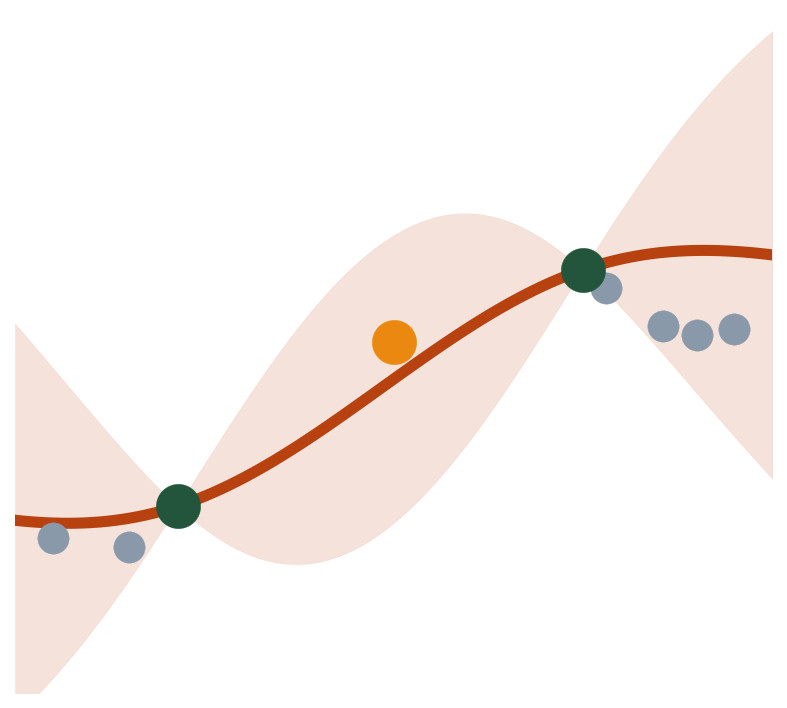
\includegraphics[width=0.5\textwidth]{graphs/predict_cknn_2}
        };
      \end{tikzpicture}
    \end{figure}

    \vspace{-0.5cm}

    \begin{figure}[h!]
      \centering
      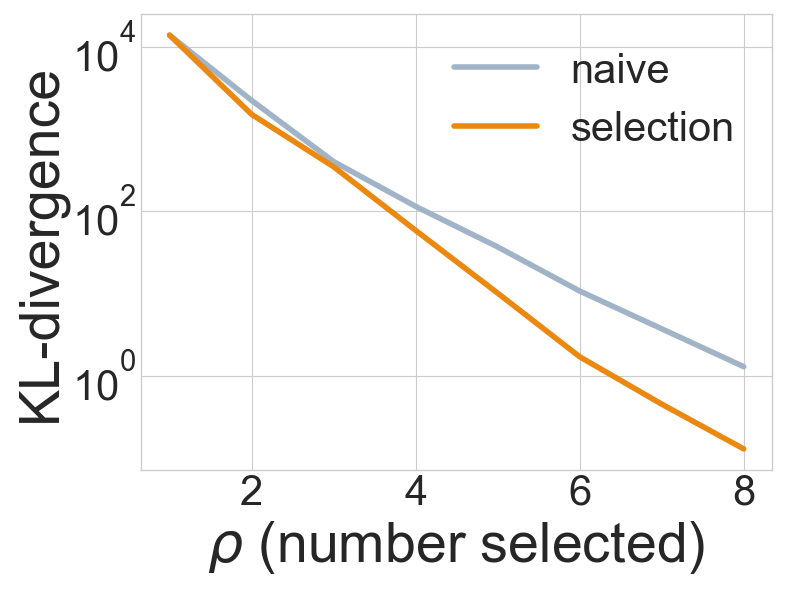
\includegraphics[width=\textwidth]{data/rho_kl-div}
    \end{figure}
  \end{column}
\end{columns}

% https://tex.stackexchange.com/questions/340058/uncovered-footnote-appears-too-early-in-beamer-presentation
\alt<3->{\footnotetext{\fullcite{schafer2020sparse}}}
{\let\thefootnote\relax\footnotetext{~ \newline ~}}
\end{frame}
\endgroup

\begin{frame}
\frametitle{GP regression by Cholesky factorization}
\framesubtitle{}
\begin{itemize}
  \item<+-> Lower triangular factor for precision:
    \( L L^{\top} = \Theta^{-1} \)
  \item<+-> Upper triangular factor for covariance:
    \( L^{-\top} L^{-1} = \Theta \)
  \item<+-> \( U = L^{-\top} \), look at submatrices:
    \begin{align*}
      \Theta &= U U^{\top} =
      \begin{pmatrix}
        U_{11} & U_{12} \\
        0 & U_{22}
      \end{pmatrix}
      \begin{pmatrix}
        U_{11}^{\top} & 0 \\
        U_{12}^{\top} & U_{22}^{\top}
      \end{pmatrix} \\
      &=
      \begin{pmatrix}
        U_{11} U_{11}^{\top} + U_{12} U_{12}^{\top} & U_{12} U_{22}^{\top} \\
        U_{22} U_{12}^{\top} & U_{22} U_{22}^{\top}
      \end{pmatrix} \\
      U_{22} &= \chol(\Theta_{22}) \\
      U_{12} &= \Theta_{12} U_{22}^{-^{\top}} \\
      U_{11} &= \chol(\Theta_{11 \mid 2})
    \end{align*}
\end{itemize}
\end{frame}

\begin{frame}
\frametitle{GP regression by Cholesky factorization}
\framesubtitle{}
\begin{itemize}
  \item<+-> Write conditional terms:
    \begin{align*}
      \E[\vec{y}_1 \mid \vec{y}_2] &= \Theta_{12} \Theta_{22}^{-1} \vec{y}_2 \\
      &= U_{12} U_{22}^{-1} \vec{y}_2 \\
      \Cov[\vec{y}_1 \mid \vec{y}_2]
        &= \Theta_{11} - \Theta_{12} \Theta_{22}^{-1} \Theta_{21} \\
      &= U_{11} U_{11}^{\top}
    \end{align*}
  \item<+-> Recall: \( U = L^{-\top} \) so \( U L^{\top} = L^{\top} U = I \)
    \begin{align*}
      \begin{pmatrix}
        U_{11} & U_{12} \\
        0 & U_{22}
      \end{pmatrix}
      \begin{pmatrix}
        L_{11}^{\top} & L_{21}^{\top} \\
        0 & L_{22}^{\top}
      \end{pmatrix}
      =
      \begin{pmatrix}
        L_{11}^{\top} & L_{21}^{\top} \\
        0 & L_{22}^{\top}
      \end{pmatrix}
      \begin{pmatrix}
        U_{11} & U_{12} \\
        0 & U_{22}
      \end{pmatrix}
      &= I \\
      \begin{pmatrix}
        U_{11} L_{11}^{\top} & U_{11} L_{21}^{\top} + U_{12} L_{22}^{\top} \\
        0 & U_{22} L_{22}^{\top}
      \end{pmatrix}
      =
      \begin{pmatrix}
        I & 0 \\
        0 & I
      \end{pmatrix}
      &= I \\
      \begin{pmatrix}
        L_{11}^{\top} U_{11} & L_{11}^{\top} U_{12} + L_{21}^{\top} U_{22} \\
        0 & L_{22}^{\top} U_{22}
      \end{pmatrix}
      =
      \begin{pmatrix}
        I & 0 \\
        0 & I
      \end{pmatrix}
      &= I
    \end{align*}
\end{itemize}

\end{frame}
\begin{frame}
\frametitle{GP regression by Cholesky factorization}
\framesubtitle{}
\begin{itemize}
  \item<+-> Reading from submatrices,
    \begin{align*}
      U_{11} &= L_{11}^{-\top} \\
      U_{22} &= L_{22}^{-\top} \\
      % U_{12} L_{22}^{\top} &= -U_{11} L_{21}^{\top} \\
      U_{12} &= -L_{11}^{-\top} L_{21}^{\top} L_{22}^{-\top}
    \end{align*}
  \item<+-> Re-write conditional terms:
    \begin{align*}
      \E[\vec{y}_1 \mid \vec{y}_2] &= U_{12} U_{22}^{-1} \vec{y}_2 \\
      &= (-L_{11}^{-\top} L_{21}^{\top} L_{22}^{-\top})
        L_{22}^{\top} \vec{y}_2 \\
      &= -L_{11}^{-\top} L_{21}^{\top} \vec{y}_2 \\
      \Cov[\vec{y}_1 \mid \vec{y}_2] &= U_{11} U_{11}^{\top} \\
      &= L_{11}^{-\top} L_{11}^{-1} \\
      \vec{e}_i^{\top} \Cov[\vec{y}_1 \mid \vec{y}_2] \vec{e}_j &=
        (L_{11}^{-1} \vec{e}_i)^{\top} (L_{11}^{-1} \vec{e}_j)
    \end{align*}
\end{itemize}
\end{frame}

\begin{frame}
\frametitle{Summary}
\framesubtitle{}
\begin{itemize}
  \item Selection algorithm for Gaussian process regression
  \item Drop-in replacement for \( k \)-th nearest neighbors
  \item Leverage GP regression for sparse Cholesky factorization
  \item Leverage Cholesky factorization for GP regression
  \item Thank you!
\end{itemize}
\end{frame}

\end{document}
